\documentclass[]{article}
\usepackage[version=3]{mhchem}
\usepackage{natbib}
\usepackage{graphicx}
\usepackage{float}
\bibliographystyle{abbrvnat}
\usepackage[colorlinks]{hyperref}
\hypersetup{
  citecolor = {blue},
}
\newcommand{\unit}[1]{\ensuremath{\, \mathrm{#1}}}

\title {Gas density-based BMP measurement\footnote{
  Recommended citation: 
Hafner, S.D.; Mortensen, J.R.; Koch, K.; Astals, S. Gas density-based BMP measurement. Standard BMP Methods document 304, version 2.0. Available online: https://www.dbfz.de/en/BMP (accessed on March XX, 2021).
\newline
  Or see \url{https://www.dbfz.de/en/BMP} for a BibTeX file that can be imported into citation management software.
}
}
\author{Sasha D. Hafner, Jacob R. Mortensen, Konrad Koch, Sergi Astals} 

\date{\today \\
\bigskip
\textit{
  Document number 304.
  File version 2.0. 
  This document is from the Standard BMP Methods collection.
    \footnote{For more information and other documents, visit \url{https://www.dbfz.de/en/BMP}. 
    For document version history or to propose changes, visit \url{https://github.com/sashahafner/BMP-methods}.}
}
}

\begin{document}
\maketitle

\section{Introduction}
By measuring BMP bottle mass loss and biogas volume, gas density can be determined, and from this, biogas composition can be calculated.
With biogas volume measurements, methane (\ce{CH4}) production and biochemical methane potential (BMP) can be determined.
This document describes the laboratory measurements needed for applying this ``GD-BMP'' (for \textbf{g}as \textbf{d}ensity) method.
Development and validation of the method is described in \citet{justesenDevelopmentValidationLowcost2019}.
For information on GD-BMP calculations, see document 204 from the Standard BMP Methods website \citep{BMPdoc204gasdens}. 

\section{Protocol}

\subsection{Required equipment and supplies}

\begin{itemize}
    \item Electronic scale
    \item Syringes and needles
    \item Manometer
    \item Typical BMP bottles and septa
    \item Incubator or heat block
\end{itemize}

The required accuracy of the scale will depend on the quantity of biogas produced. 
Generally, stated accuracy\footnote{
  Manufacturers often report accuracy as ``linearity''. 
  Note that accuracy is not the same as ``readability'', which is the smallest value that can be read. 
} of the scale should be 30 mg for every g of substrate volatile solids (VS) used, or better (smaller)\footnote{
  For example, with 2 g of substrate VS added to each bottle, scale accuracy stated by the manufacturer must be 60 mg or better (e.g., 50 mg would be sufficient).
}.
As described below, the precision and stability of the scale is checked as part of the protocol.

A simple closed U-tube manometer or an inexpensive electronic manometer is sufficient for determining that post-venting headspace pressure is close to atmospheric.
A U-tube manometer can be made with some plastic tubing filled with water and a simple valve (made, e.g., by folding flexible tubing).

It is best to have several sizes of syringes, in order to have high relative precision in volume measurements when biogas production is both high and low.
Ideally the largest syringe will be large enough to measure the largest volume of biogas produced in a single interval.\footnote{
  Biogas production rate depends on substrate and inoculum characteristics, and is best estimated from previous experiments.
  For microcrystalline cellulose, typical production early in a test may be 200 to 300 mL biogas per g VS over one day. 
  With 2 g substrate VS then, syringe volume would ideally be more than 600 mL (perhaps 1 L), but even a 150 mL syringe could be sufficient with multiple emptying cycles.
}
But large syringes are expensive, and not necessary.
Instead, a single small syringe can be used multiple times to remove the biogas from a single bottle in a single interval.
But this approach requires that the manometer is directly connected to the syringe and there is a valve between the syringe and the bottle.
%%Videos showing this approach are available (INFO NEEDED).

An incubator or temperature-controlled room is needed to keep bottles at the desired test temperature, e.g., 37$^\circ$C.
A water bath is not recommended because water on a bottle surface will affect its weight.
Incubation of the bottles in heated air (or possibly in heat blocks) is preferable.
Ideally, venting and weighing should be done inside a temperature-controlled room, so bottles are always at the incubation temperature and the headspace temperature--needed for calculations--is known.  
However, the effect of headspace temperature error on accuracy is very small, so this is not required.

\subsection{Setup}
During setup, inoculum and substrate are added to bottles, and the headspace of each bottle is flushed to remove \ce{O2} and ensure anaerobic conditions. 
With the GD-BMP method, pure \ce{N2} is preferred for flushing over mixtures containing \ce{CO2}.\footnote{
  Flushing gas results in a (generally small) error because its density may differ from produced biogas density (the density of \ce{N2} is identical to a \ce{CH4}:\ce{CO2} mixture with 58\% \ce{CH4} and 42\% \ce{CO2}, and higher than a mixture with more \ce{CH4}) but this can be corrected in calculations \citep{justesenDevelopmentValidationLowcost2019}. 
When flushing, be sure to avoid bubbling the gas through the inoculum/substrate mixture to minimize \ce{CO2} stripping.
}
Bottles are then weighed and placed in an incubator.

\subsubsection{Step-by-step instructions}
\begin{enumerate}
  \item Carefully set up and level the scale on a stable surface (following manufacturer's instructions) and check its accuracy with a weight set. 
      It is particularly important that the actual accuracy is close to reported accuracy when weighing an object with a mass close to the total mass of a BMP bottle and its contents. 
      For a scale with a reported accuracy of 50 mg, for example, this could be checked by taring the scale with a full bottle or equivalent mass, and adding a 50 mg weight.
    \item Add the required mass of inoculum, substrate, and other additions (e.g., a trace element solution) to each labeled bottle and seal with a septum and cover. 
      Determination of the quantity of material added by mass difference is the recommended approach: tare scale with bottle, add approximately the desired quantity, wipe any material from near the mouth of the bottle, and finally determine the actual quantity from the scale reading. 
      Note that the scale used here does not need to be the same scale used for determining mass loss (see ``Incubation and sampling'', below).
    \item Flush the bottle headspace to remove \ce{O2}. 
      A simple approach is to use a needle attached to a flow meter (e.g., a rotameter), a pressure regulator (to ensure low pressure), and a gas cylinder (generally with \ce{N2}) with plastic tubing, along with a separate needle for venting. 
      Minimize \ce{CO2} removal by flushing for only 3 to 4 headspace volume exchanges. 
      Ensure that the flushing gas does not bubble through the liquid in the bottle (needle should not be submerged) to avoid \ce{CO2} removal. 
      Allow the pressure in each bottle’s headspace to equilibrate with atmospheric pressure before removing the venting needle.
    \item Make 3 ``water control'' bottles that contains only water. 
      They should be the same size and weigh about as much as the other BMP bottles. 
      These bottles should never be vented; they are used to check the stability of the scale and it is essential that they do not lose any mass.
    \item Weigh each bottle and record as ``initial mass''. 
      Repeat this initial weighing in order to minimize the chance of a recording error, because calculations of cumulative \ce{CH4} production at all timepoints require an accurate initial mass measurement.
      If there is a discrepancy between these two initial measurements, weigh again to determine the correct mass.
      It is important that the only change in bottle mass after this time is due to biogas removal.
      Bottles should be kept clean, and labels should not be added after this time, for example.
    \item Place bottles in incubator set at the test temperature.
\end{enumerate}

\subsection{Incubation and sampling}
Bottles are removed from the incubator occasionally to vent and weigh in what is here referred to as a ``sampling event''. 
Biogas temperature affects water vapor content. 
To minimize uncertainty in the headspace temperature used in calculations, the time that bottles spend outside the incubator should be short, and the same procedure and timing should be followed for each sampling event. 

The accuracy of the GD-BMP method is affected only slightly by variation in headspace pressure, and it is possible to correct for leakage of biogas. 
However, for safety (to avoid exploding bottles), for maximum precision, and to minimize possible effects of high \ce{CO2} dissolution, total headspace pressure (absolute) should be kept below about 300 kPa (200 kPa (2 bar) gauge pressure). 
Bottle pressures can be estimated from headspace and vented biogas volume.\footnote{
  Or measured directly before venting if an electronic manometer is used.
  However, as with headspace temperature, the effect of uncertainty here is very small.
}

Unlike headspace conditions, the temperature and pressure of biogas at the time of volume measurement is important to determine in order to standardize the volume.
When using syringes, it is reasonable to assume that the syringe and gas inside are approximately at the ambient temperature.
With a manometer, the pressure can be kept nearly identical to the ambient value.
Therefore ambient pressure and temperature (room pressure and temperature) must be determined or, if necessary, estimated.
Absolute pressure can now be measured using barometer apps on many smart phones.
Alternatively, pressure can be determined from public meteorological data (from a closeby weather station), with corrections for elevation if necessary.

\subsubsection{Step-by-step instructions} \label{sec:steps}
\begin{enumerate}
    \item Measure and record the room temperature and pressure at which biogas volume will be determined.
    \item Remove the 3 water control bottles from the incubator and weigh them to confirm scale consistency. 
      If the results are the same as the initial masses (within the expected accuracy) proceed, otherwise, identify and address the problem with the scale or replace the scale if necessary.
      If the problem cannot be resolved, proceed and later correct mass results for scale drift.\footnote{
        Correction is done by subtracting the average apparent mass gain in the water control bottles from all mass measurements made during that particular sampling event. 
        For example, if both water controls weighed 0.1 g more on day 4 than at the start, the measured masses of all bottles from day 4 should be adjusted downward by 0.1 g.
      }
    \item Remove a single set of replicates from the incubator (e.g., the three replicates for cellulose).
    \item Always starting with the same replicate (e.g., ``1'' or ``a'')\footnote{
        If this is done the effect of gradual headspace cooling on measurement error (expected to be minor) can be confirmed by comparing BMP from individual replicates across all substrates.
      } gently swirl the bottle for at least 10 s to mix the contents and encourage \ce{CO2} equilibration between solution and headspace. 
      During swirling, avoid contact between the liquid and the septum.\footnote{
        If the septum becomes contaminated with reacting material, a small amount may be pushed out during venting, which will result in error in the determination of mass loss.
        Generally it is easy to avoid this problem, but if it does occur, be sure to note the occurence to help with interpretation later.
        If the loss is small and there is no noticable difference among the replicates, the problem could be ignored. 
        Otherwise, data from this replicate should be discarded.
      }
    \item Weigh the bottle and record the result as pre-venting mass.
    \item Vent the bottle using a syringe and measure biogas volume (see Section \ref{sec:volmeas}).
      Use the manometer to ensure that the pressure of both removed biogas and biogas remaining in the bottle headspace after venting pressure is close to atmospheric (gauge pressure = 0 $\pm3$ kPa).
    \item Weigh the bottle after venting, and record the result as post-venting mass. 
    \item Proceed to the next replicate (e.g., ``2'' or ``b'') and repeat steps 4 - 7.
    \item After all replicates have been mixed, weighed, vented, and weighed again, place the bottles back in the incubator.
    \item Proceed to the next set of replicates (e.g., the three replicates for substrate ``food waste A'') and repeat steps 3 - 9.
\end{enumerate}

This sequence of steps is shown in Fig. \ref{fig:steps}.

\begin{figure}
  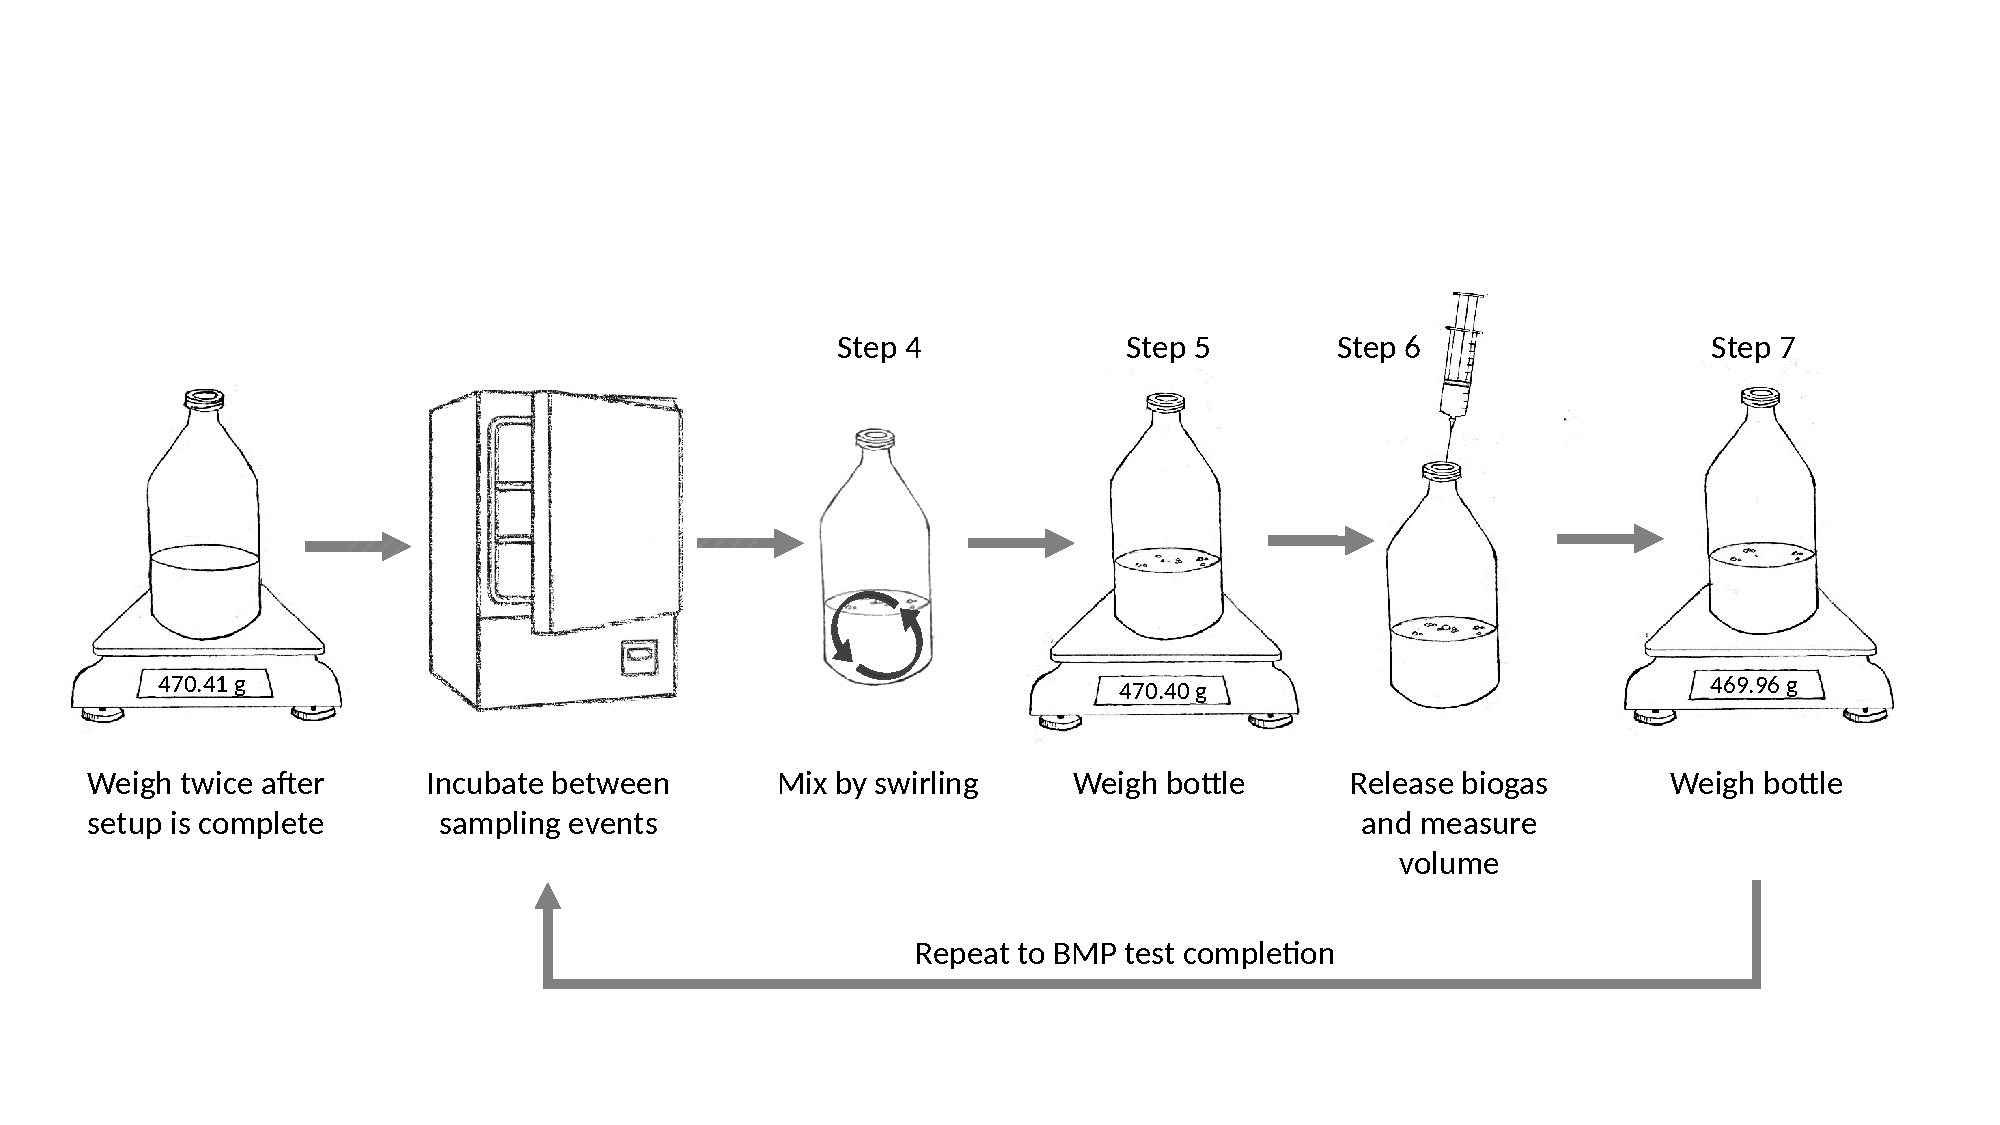
\includegraphics[width=\textwidth]{figs/GD_steps.pdf}
  \caption{The data collection steps required for GD-BMP measurements. Step numbers match those listed in the text, and are repeated for each sampling event. For details on volume measurement (step 6) see Section \ref{sec:volmeas}.}
  \label{fig:steps}
\end{figure}


\subsection{Volume measurement} \label{sec:volmeas}
Volume measurement in Section \ref{sec:steps} should take place at ambient pressure, in order to later convert the measurement to standardized volume.
This task can be done very simply with an inexpensive plastic syringe and a simple U-tube manometer, as long as the capacity of the syringe (maximum volume) is greater than the quantity of biogas produced in any sampling interval.
Unfortunately, typical small syringes ($\le$ 150 mL) are generally not large enough, and large syringes (e.g., 1 L) are expensive.
There are at least two solutions:
\begin{itemize}
  \item Use multiple syringes to remove accumlated gas all at one time.
  \item Use a simple manometer and a three-way valve to measure accumulated gas in steps. This is shown in Fig. \ref{fig:utube}.
\end{enumerate}

The first approach is straightforward, but handling three or more syringes with only two hands is challenging.
The second requires construction of a simple U-tube manometer system, shown in Fig. \ref{fig:utube}, and its construction and use is described here.
The manometer should be made from flexible plastic tubing, large enough to avoid problems due to adhension.\footnote{Clear polyvinyl chloride (PVC) tubing with a 3/8 inch inner diameter works well.}
It is filled with water to the level shown by ii in Fig. \ref{fig:utube}, and clamped at location i to create a \textit{closed}-tube manometer.\footnote{This is essential. An open-tube manometer would lose its water under even moderate pressure.}
Smaller diameter tubing (iii in Fig. \ref{fig:utube}) can be used to connect to the three-way valve (A, B, C).\footnote{Plastic valves sometimes called "disposable medical three-way stopcock valves" are inexpensive and work well for this task.}
When in use, the system is connected to a BMP bottle via a needle (iv in Fig. \ref{fig:utube})\footnote{21 gauge/0.8 mm works well.}.
A syringe is connected through tubing to the valve (v in Fig. \ref{fig:utube})
This connection should be easy to disconnect, in order to vent biogas.
With this system, the following steps are used for each bottle.
The capital letters (labeled with A, B, C) and small Roman numerals (i, ii, ...) refer to the labels in Fig. \ref{fig:utube}.
\begin{enumerate}
  \item With syringe disconnected (around location v), check that water levels at ii are equal. Equilibrate closed end by removing and replacing clamp at i if necessary.
  \item Turn valve so connection B-C is open (A closed) and allow accumulated biogas to flow under pressure to no more than ca. 80 or 90\% of syringe capacity.
  \item Turn valve so connection A-C is open (B closed) and adjust syringe plunger position so the water levels at ii are equal. Read and record volume.
  \item Disconnect syringe at v, push out biogas, and return to step 1, repeating until all excess accumulated biogas has been removed, i.e., when headspace pressure is equal to atmospheric (determined by completely opening valve, A-B-C open).
\end{enumerate}

\begin{figure}
  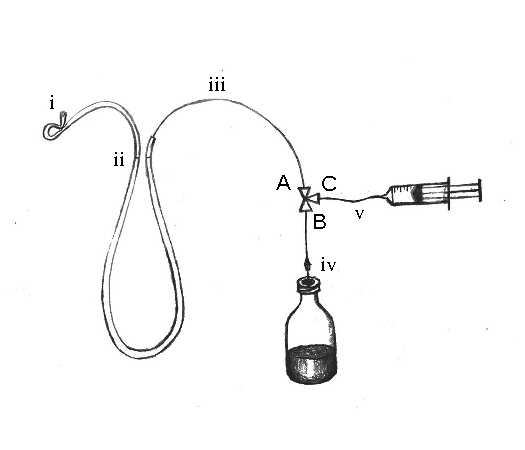
\includegraphics[]{figs/GD_utube.pdf}
  \caption{The U-tube manometer/3-way valve approach to measuring biogas volume. See Section \ref{sec:volmeas} for an explanation.} 
  \label{fig:utube}
\end{figure}

\subsection{Testing}
The GD-BMP method requires accurate determination of gas volume and bottle mass loss.
It is important that any new setup is tested.
Fortunately, ambient air can be used as a standard.
To test the system, simply force a volume (more than ca. 20\% of a bottle headspace is difficult to add) into an empty bottle, and proceed with the measurement steps given above. 
Calculate apparent density based on bottle mass loss and volume of gas removed.\footnote{This volume may be smaller than the volume thought to be added because of leakage during addition or removal of the syringe.}
The value should be within 10\% (or better, 5\%) of the density for the known ambient pressure and temperature.\footnote{Humidity effects are small around room temperature (assuming $\le$ 25$^\circ$C).}

\section{Calculations}
See document 204 from the Standard BMP Methods website \citep{BMPdoc204gasdens} for a detailed description of calculations. 


\bibliography{bib}

\end{document}
